% Chapter Template
\chapter{Ensayos y Resultados} % Main chapter title
En este capítulo se expone cuales fueron las pruebas realizadas para determinar que el sistema funciona en forma correcta.
\label{Chapter4} % Change X to a consecutive number; for referencing this chapter elsewhere, use \ref{ChapterX}

\section{Banco de pruebas}
Para poder simular el comportamiento de un sensor de temperatura y la descarga de una batería. Se implemento una placa básica la cual ya fue vista en el capitulo 3.2, que para facilidad del lector volvemos a mostrarla en la siguiente figura \ref{fig:placa_básica}, la cual consta de dos potenciómetros, que permiten simular la variación de estos dispositivos. Sobre la misma se conecto un conversor RS232 a TTL, para lograr la integración del módem GPRS \emph{SIM800L}.

\begin{figure}[h]
  \centering
  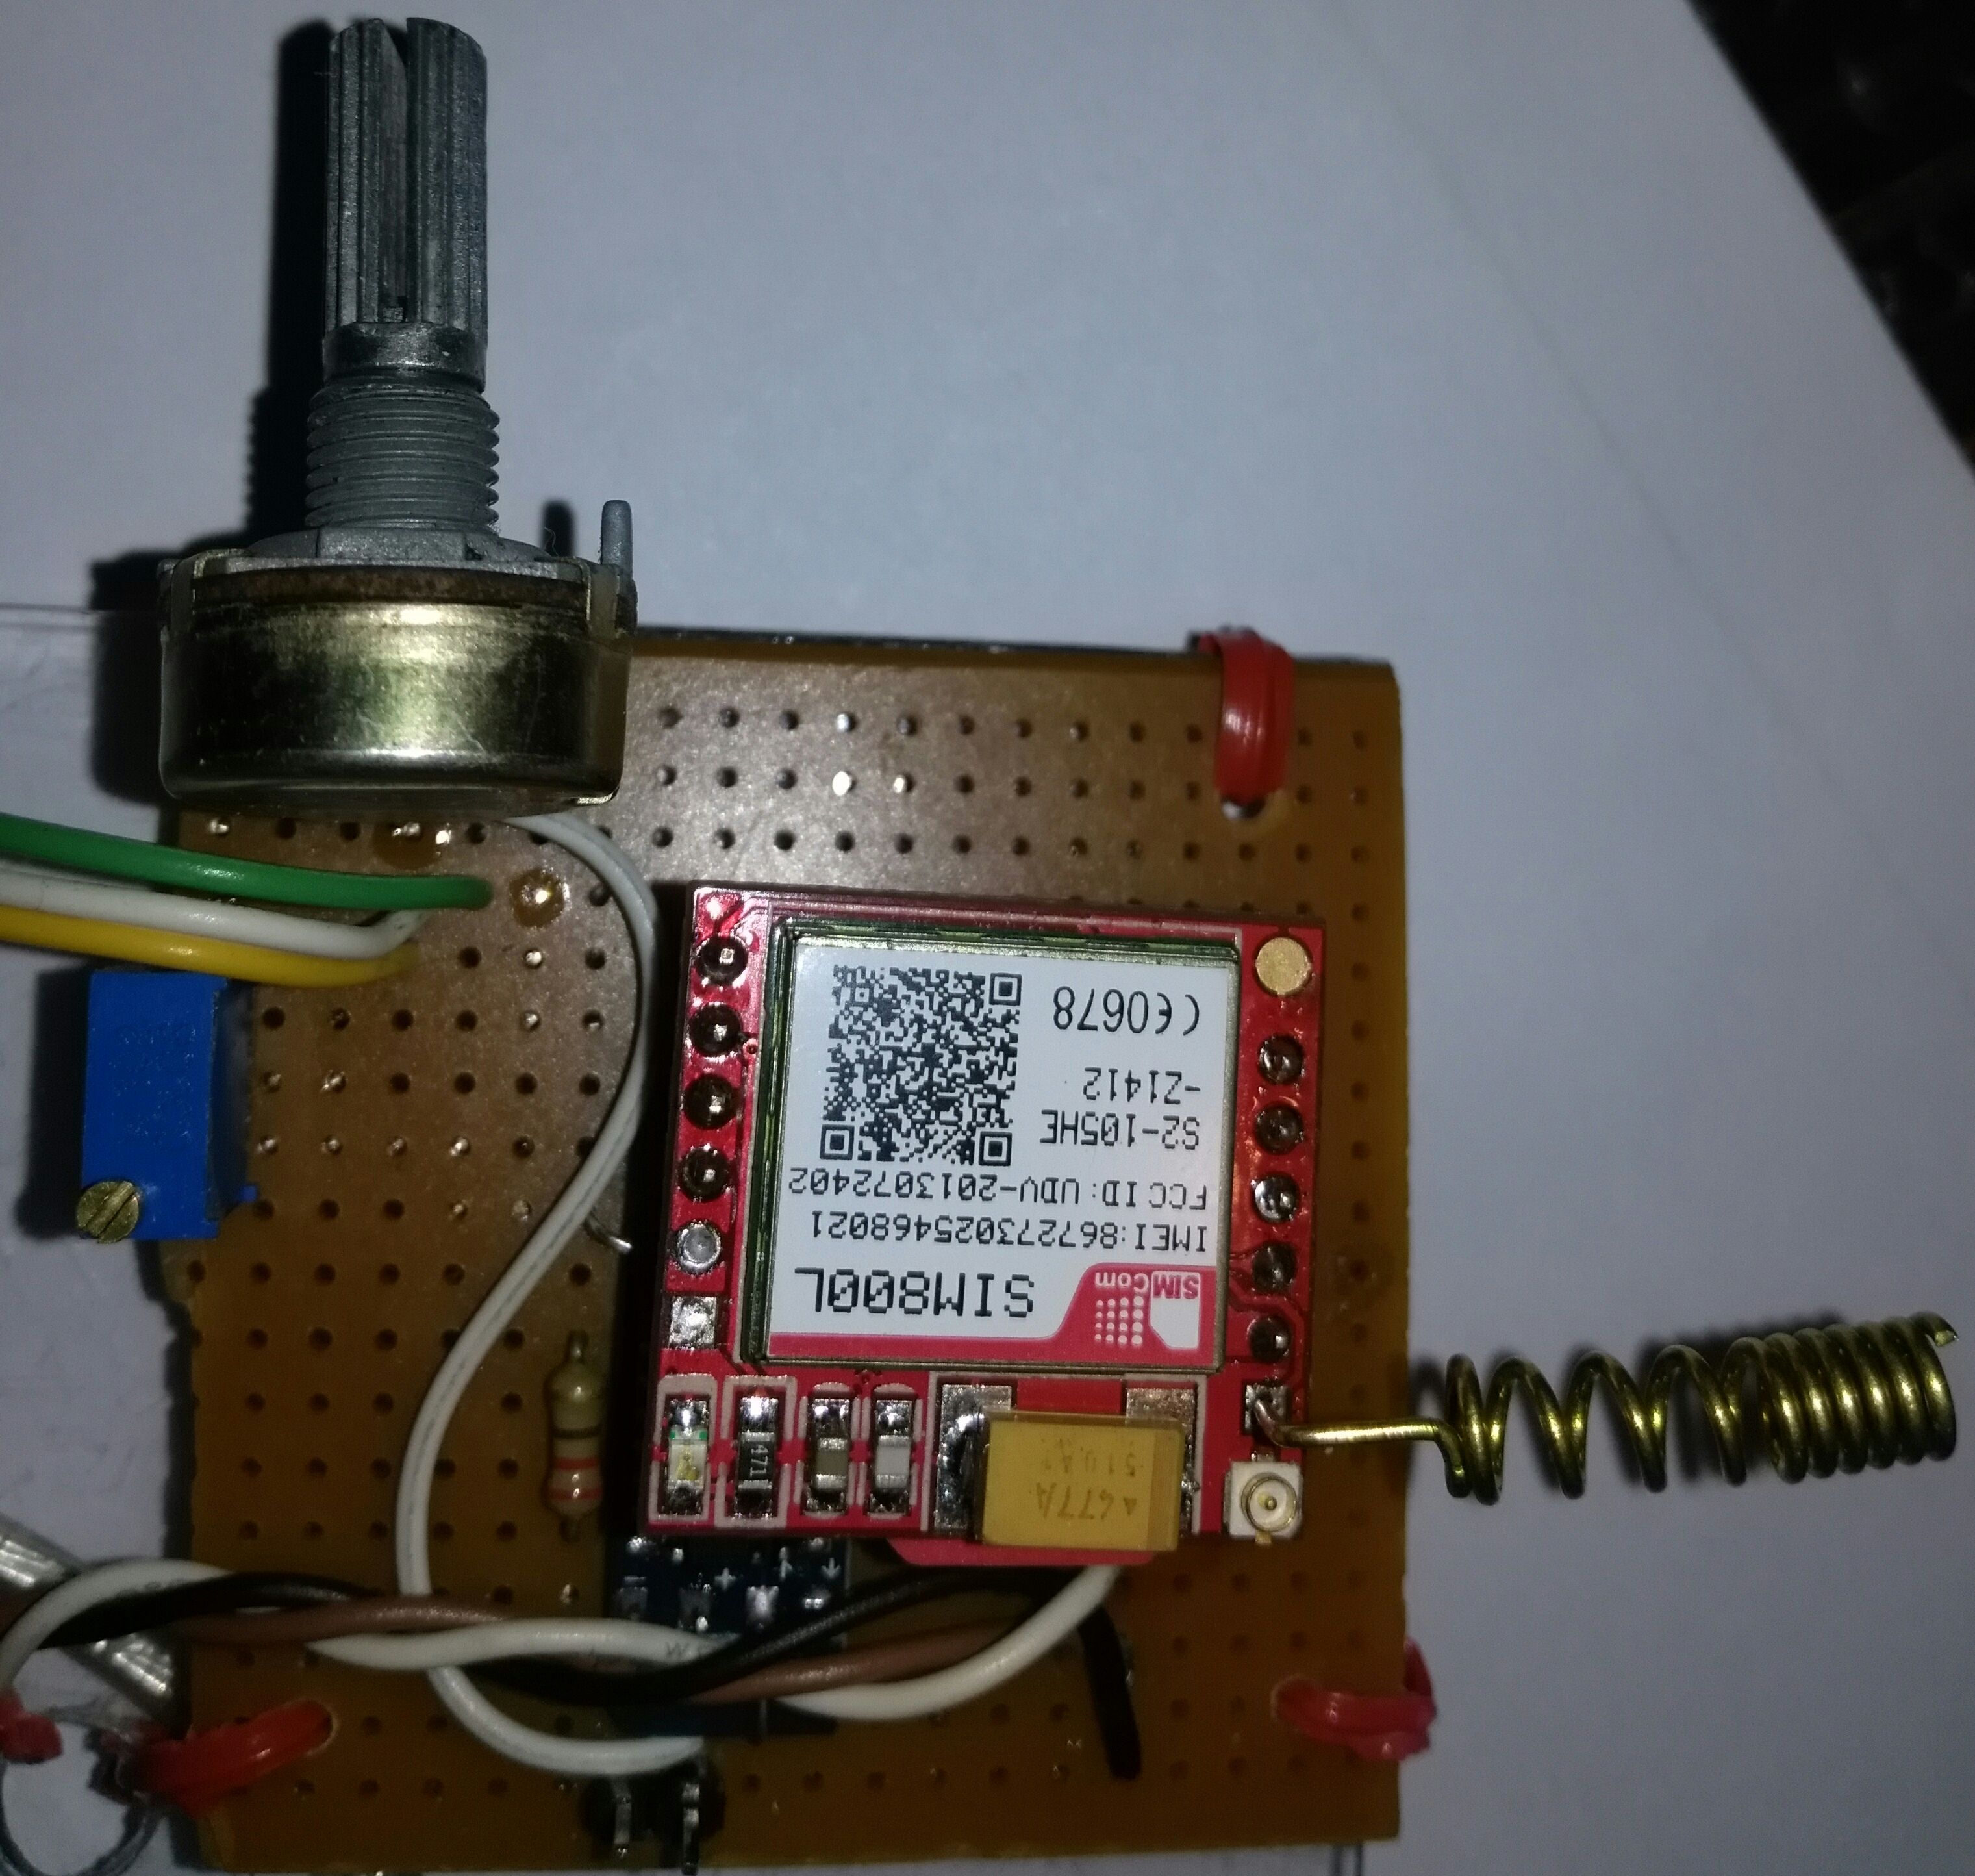
\includegraphics[scale=.03]{./Figures/placa_basica.jpg}
  \caption{Placa de simulación de temperatura y estado de la batería con el modulo SIM800l integrado.}
  \label{fig:placa_básica}
\end{figure}

Todo esto se integra la Plataforma de la CIAA-NXP, véase figura \ref{fig:prototipo}, para verificar el correcto funcionamiento del firmware desarrollado.

\begin{figure}[h]
  \centering
  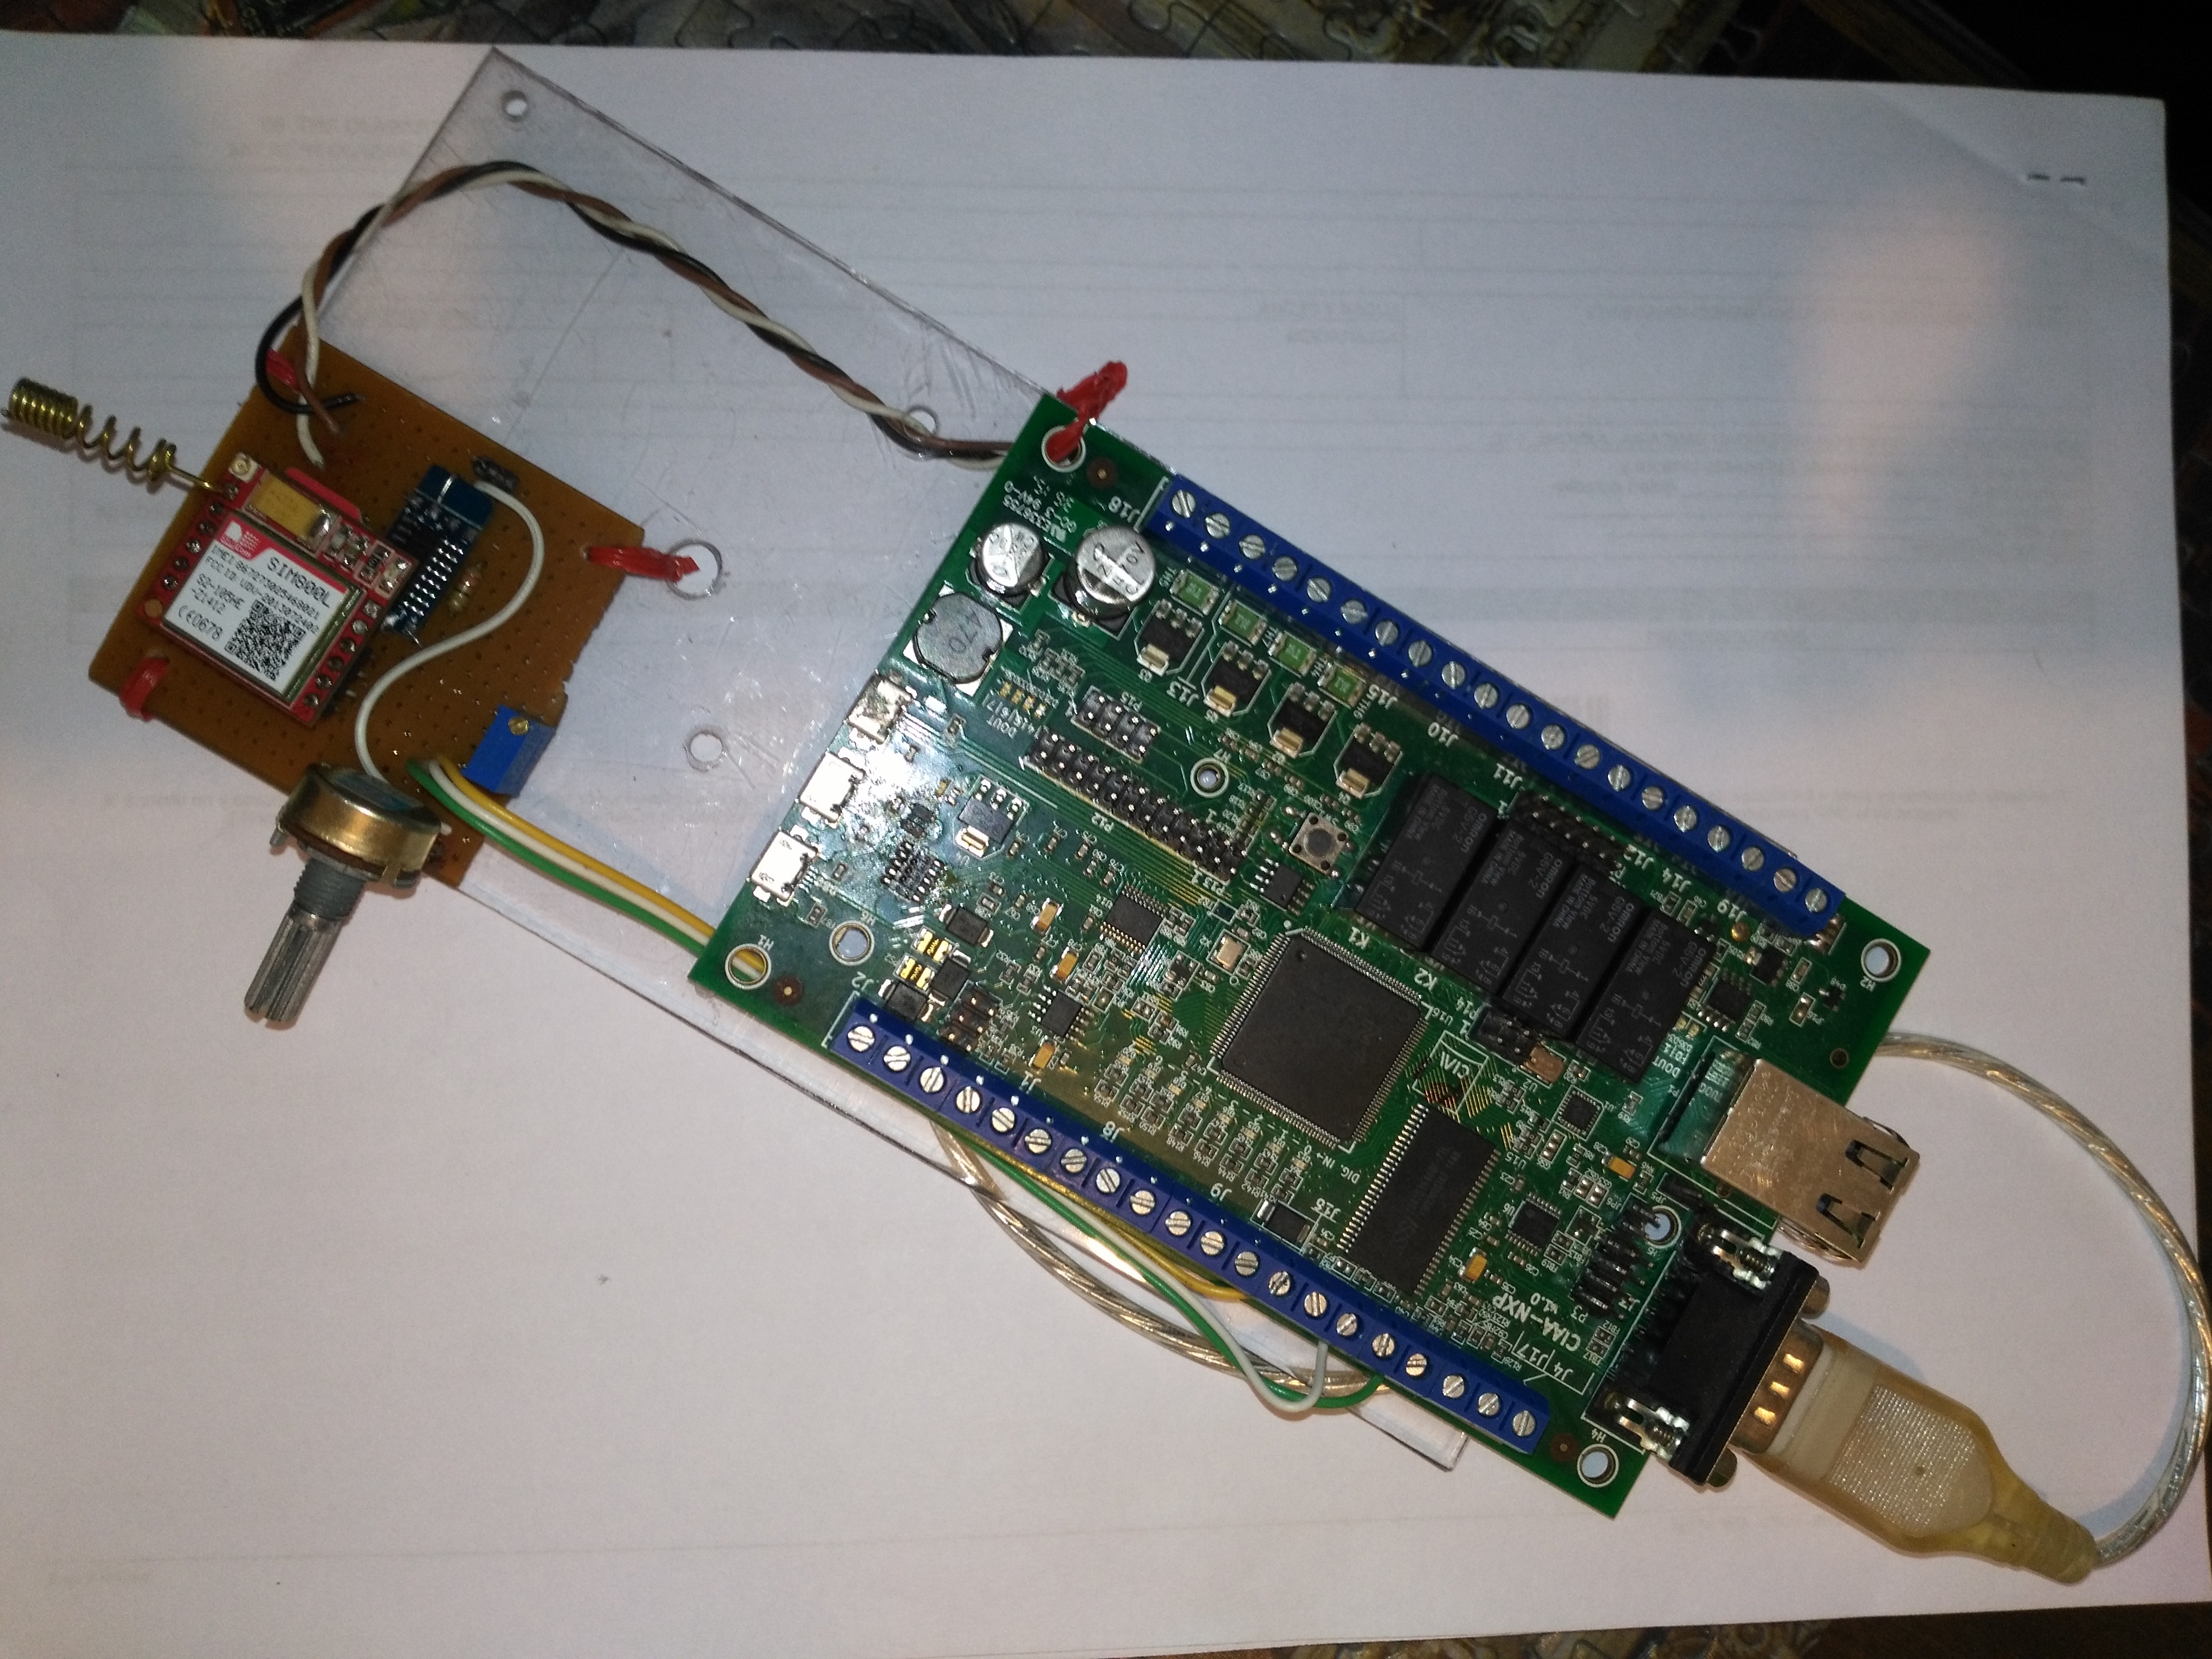
\includegraphics[scale=.04]{./Figures/prototipo.jpg}
  \caption{Placa básica integrada con la CIAA-NXP.}
  \label{fig:prototipo}
\end{figure}

\section{Configuraciones para la PC}

Para la realización de los ensayos, comenzamos configurando la PC en forma adecuada. Para ello en la siguiente figura \ref{fig:hw_pc} vamos a ver como configurar en Linux la interfaz de red. Es importante destacar que dichos comandos son ejecutados con el permiso se súper usuario, \emph{root}.

\begin{figure}[h]
  \centering
  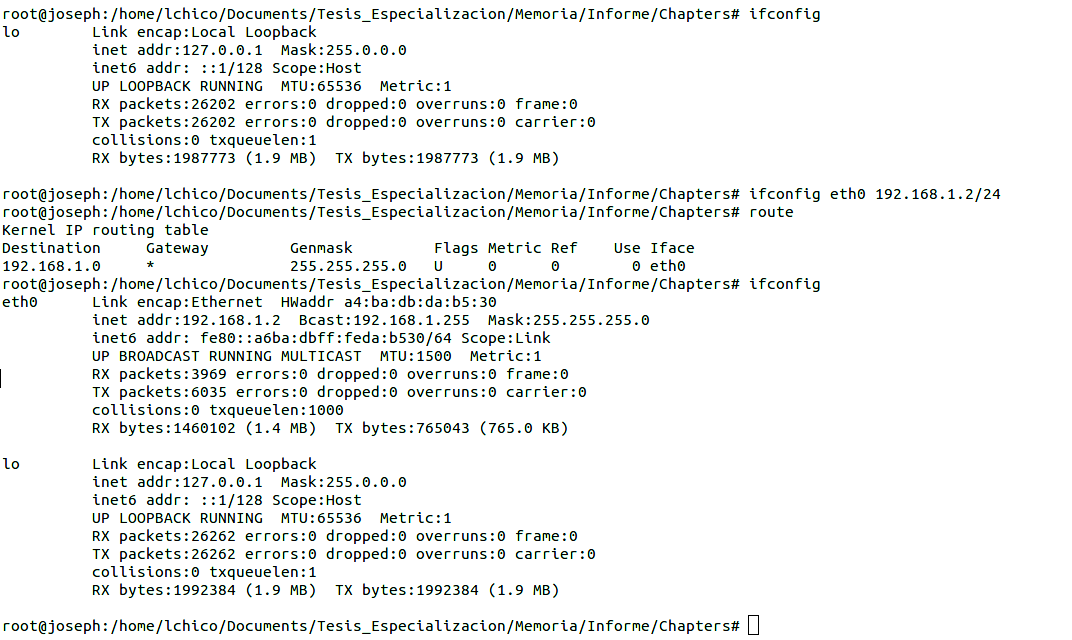
\includegraphics[scale=.35]{./Figures/config_net_console.png}
  \caption{Configuración de una red estática para la interfaz Ethernet.}
  \label{fig:hw_pc}
\end{figure}

Una vez que tenemos la configuración de red adecuada vamos a proceder a dirigirnos a un navegador web. Y como vemos en la imagen \ref{fig:web_monitoreo} ingresamos el numero de ip correspondiente al dispositivo de control, la cual es: 192.168.1.11 

\begin{figure}[h]
  \centering
  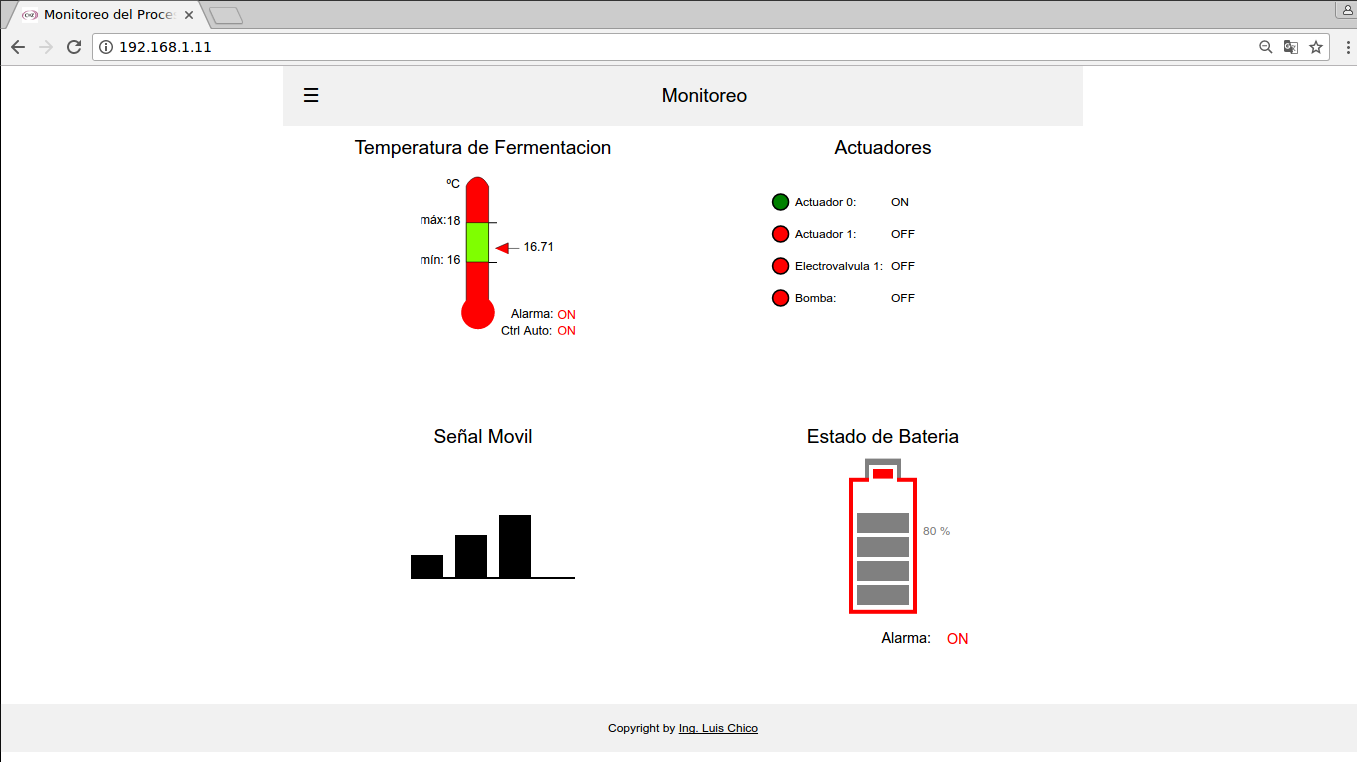
\includegraphics[scale=.25]{./Figures/web_monitoreo.png}
  \caption{Pantalla principal de la web de monitoreo.}
  \label{fig:web_monitoreo}
\end{figure}

En esta pantalla vamos a tener toda la información correspondiente al sistema. Arriba a la izquierda podemos ver el estado de la temperatura, con sus rangos máximos y mínimos seteados. Y debajo de dicho termómetro podemos ver si esta activada: la alarma y el control automático.

Luego arriba y a la derecha podemos ver los estados de los actuadores, la electroválvula y la bomba. Estos le permiten al cliente controlar en forma remota dos actuadores y el sistema correspondiente a la bomba de refrigeración con la electroválvula asociada. El sensor de temperatura permitirá informarle al sistema de control automático cuando debe actuar acorde a los rangos establecidos, esto solo en el caso de estar activado dicho control automático. 

Abajo a la izquierda tenemos en nivel de señal correspondiente al módem GSM, mediante el cual podremos saber si la cobertura de señal de la red de telefonía móvil esta en condiciones de operar y permitirnos el servicio de alertas mediante mensajes SMS. 

Finalmente abajo a la derecha tenemos el estado de la batería, el cual va a permitir al sistema continuar en funcionamiento en caso de un corte de energía. El principal uso de este será mantener la posibilidad de enviar un mensaje SMS notificando el corte de energía.

\section{Verificación del sistema web embebido} 
De lo explicado en la sección anterior, se procederá a navegar por el menú, véase figura \ref{fig:web_menus_num}, las diferentes configuraciones para constatar de que todo el sistema esta funcionando en forma correcta. Al presionar donde dice menú, obtendremos las opciones de configuración. Donde:

\begin{figure}[h]
  \centering
  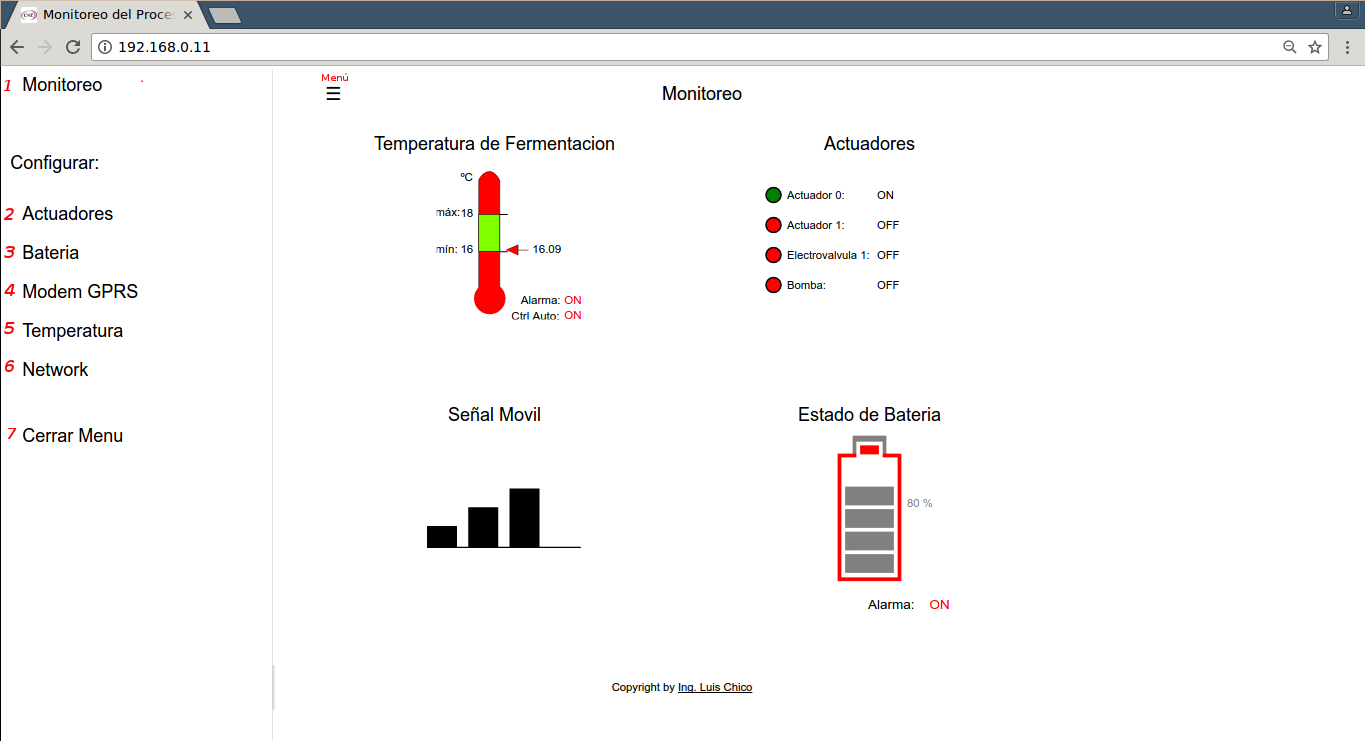
\includegraphics[scale=.25]{./Figures/web_menus_num.png}
  \caption{Opciones del al presionar sobre el menú desplegable.}
  \label{fig:web_menus_num}
\end{figure}



\begin{description}
  \item[1. Monitoreo:] Nos dirige a la pantalla principal, donde podemos ver el estado del sistema. figura \ref{fig:web_monitoreo}.
  \item[2. Actuadores:] Podemos setear en forma manual el estado de los mismos. figura \ref{fig:web_act}.
  \item[3. Batería:] Aquí podrá setear la alarma debido al nivel de descarga de batería que configuremos. Esta enviara un SMS indicando el estado. figura \ref{fig:web_bat}.
  \item[4. Módem GPRS:] En este menú podremos configurar 2 personas a quienes serán enviadas las alertas debido al accionar de alguna alarma.\ref{fig:web_Modem}.
  \item[5. Temperatura:] Aquí se configura el rango de temperatura, la alarma correspondiente y si deseamos activar el control automático de la misma. De estar activado, actuará en forma automática sobre la bomba y la electroválvula para mantener la temperatura dentro de dicho rango. figura \ref{fig:web_temp}.
  \item[6. Network:] Aqui se configura los parametros de la red, IP, mascara de red y puerta de enlace. figura \ref{fig:cfg_net}.
  \item[7. Cerrar Menú:] Esta opción cerrar el menú, permitiendo quedarse en la sección que estaba antes de presionar en menú.
\end{description}

\begin{figure}[h]
  \centering
  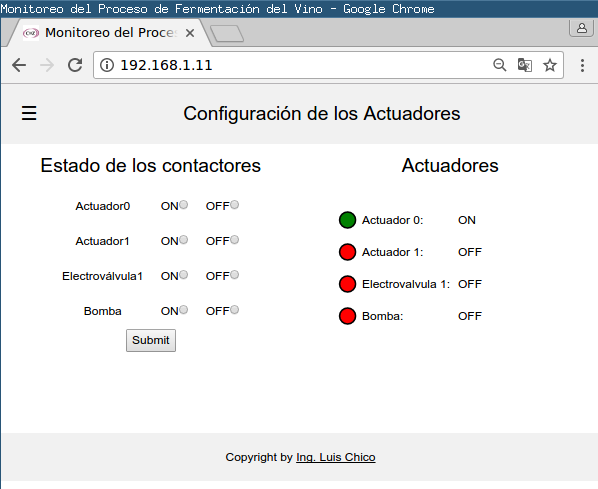
\includegraphics[scale=.25]{./Figures/config_act.png}
  \caption{ Activar/Desactivar actuadores.}
  \label{fig:web_act}
\end{figure}

\begin{figure}[h]
  \centering
  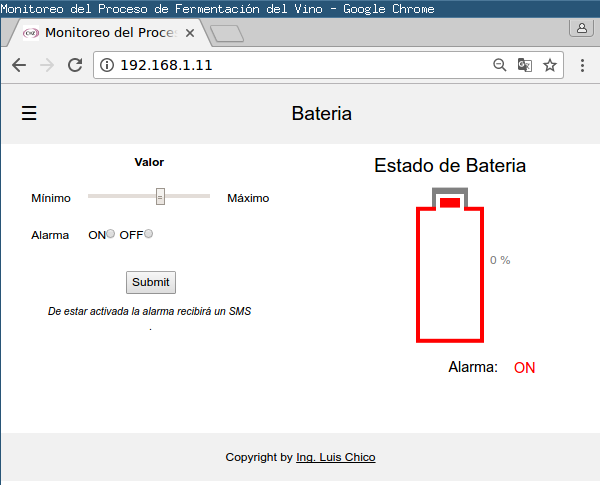
\includegraphics[scale=.25]{./Figures/config_bat.png}
  \caption{Configurar nivel de descarga para accionar la alerta por batería baja.}
  \label{fig:web_bat}
\end{figure}
\begin{figure}[h]
  \centering
  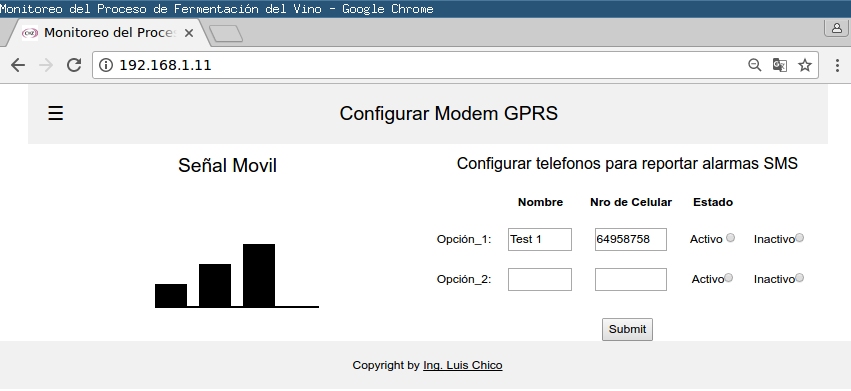
\includegraphics[scale=.25]{./Figures/config_Modem.png}
  \caption{Configuración de los celulares de quienes van a recibir las alarmas por SMS.}
  \label{fig:web_Modem}
\end{figure}
\begin{figure}[h]
  \centering
  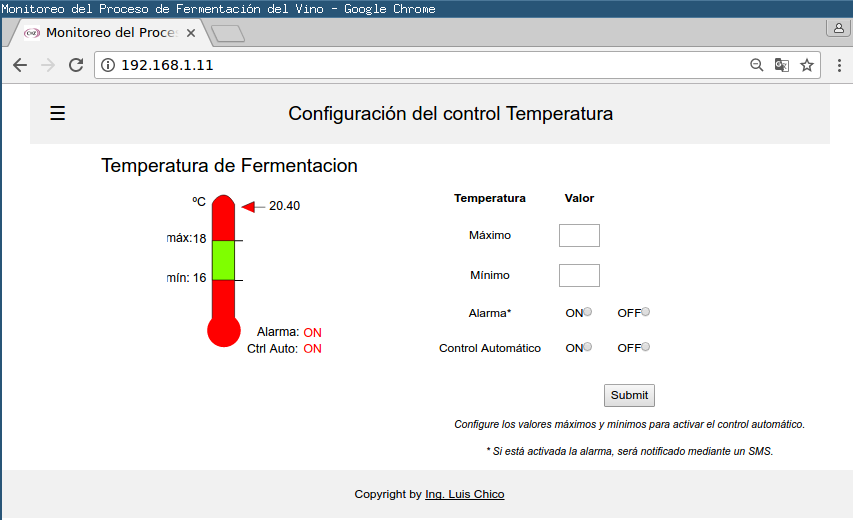
\includegraphics[scale=.25]{./Figures/config_temp.png}
  \caption{Configuración del rango de temperatura y activación del estado de control automático y alarma.}
  \label{fig:web_temp}
\end{figure}
\begin{figure}[h]
  \centering
  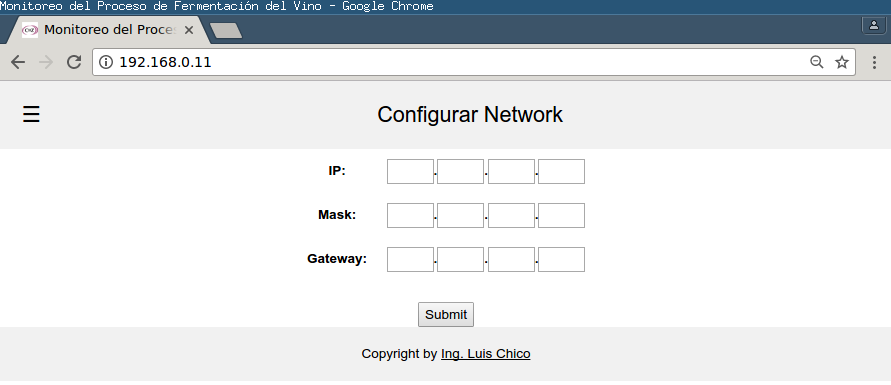
\includegraphics[scale=.25]{./Figures/config_network.png}
  \caption{Formulario de configuración de IP, mascara y puerta de enlace.}
  \label{fig:cfg_net}
\end{figure}



%----------------------------------------------------------------------------------------
%	SECTION 1
%----------------------------------------------------------------------------------------

\section{Pruebas funcionales del hardware}
\label{sec:pruebasHW}

Una vez recorrido todas las opciones que permite la interfaz web y verificar que el comportamiento haya sido el esperado. Se procede interactuar con el sistema, por medio de alteraciones generadas a través de los potenciómetros que representaran la temperatura y el estado de la batería.

Estando activado el control automático y al simular un incremento de temperatura, se comprobó que al exceder la temperatura máxima inicio en forma automática la bomba que permite la circulación del refrigerante y la activación de la electroválvula que interviene sobre el tanque que estamos monitorizando. En la web no muestra figura \ref{fig:auto_control_active}. y dado su respectiva alerta mediante un SMS como vemos en la figura \ref{fig:sms_min_max_bat}

\begin{figure}[h]
  \centering
  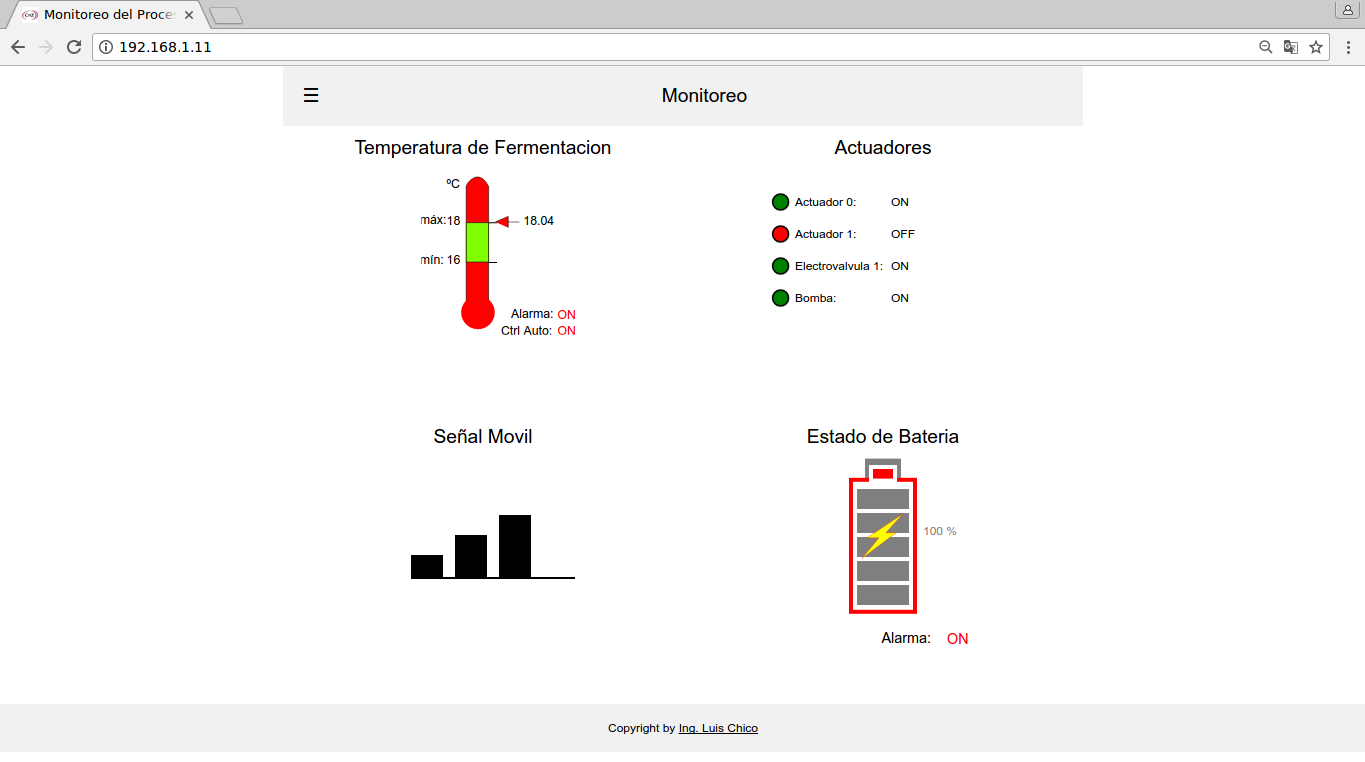
\includegraphics[scale=.25]{./Figures/auto_control_active.png}
  \caption{Activación por control automático debido a temperatura elevada.}
  \label{fig:auto_control_active}
\end{figure}


\begin{figure}[h]
  \centering
  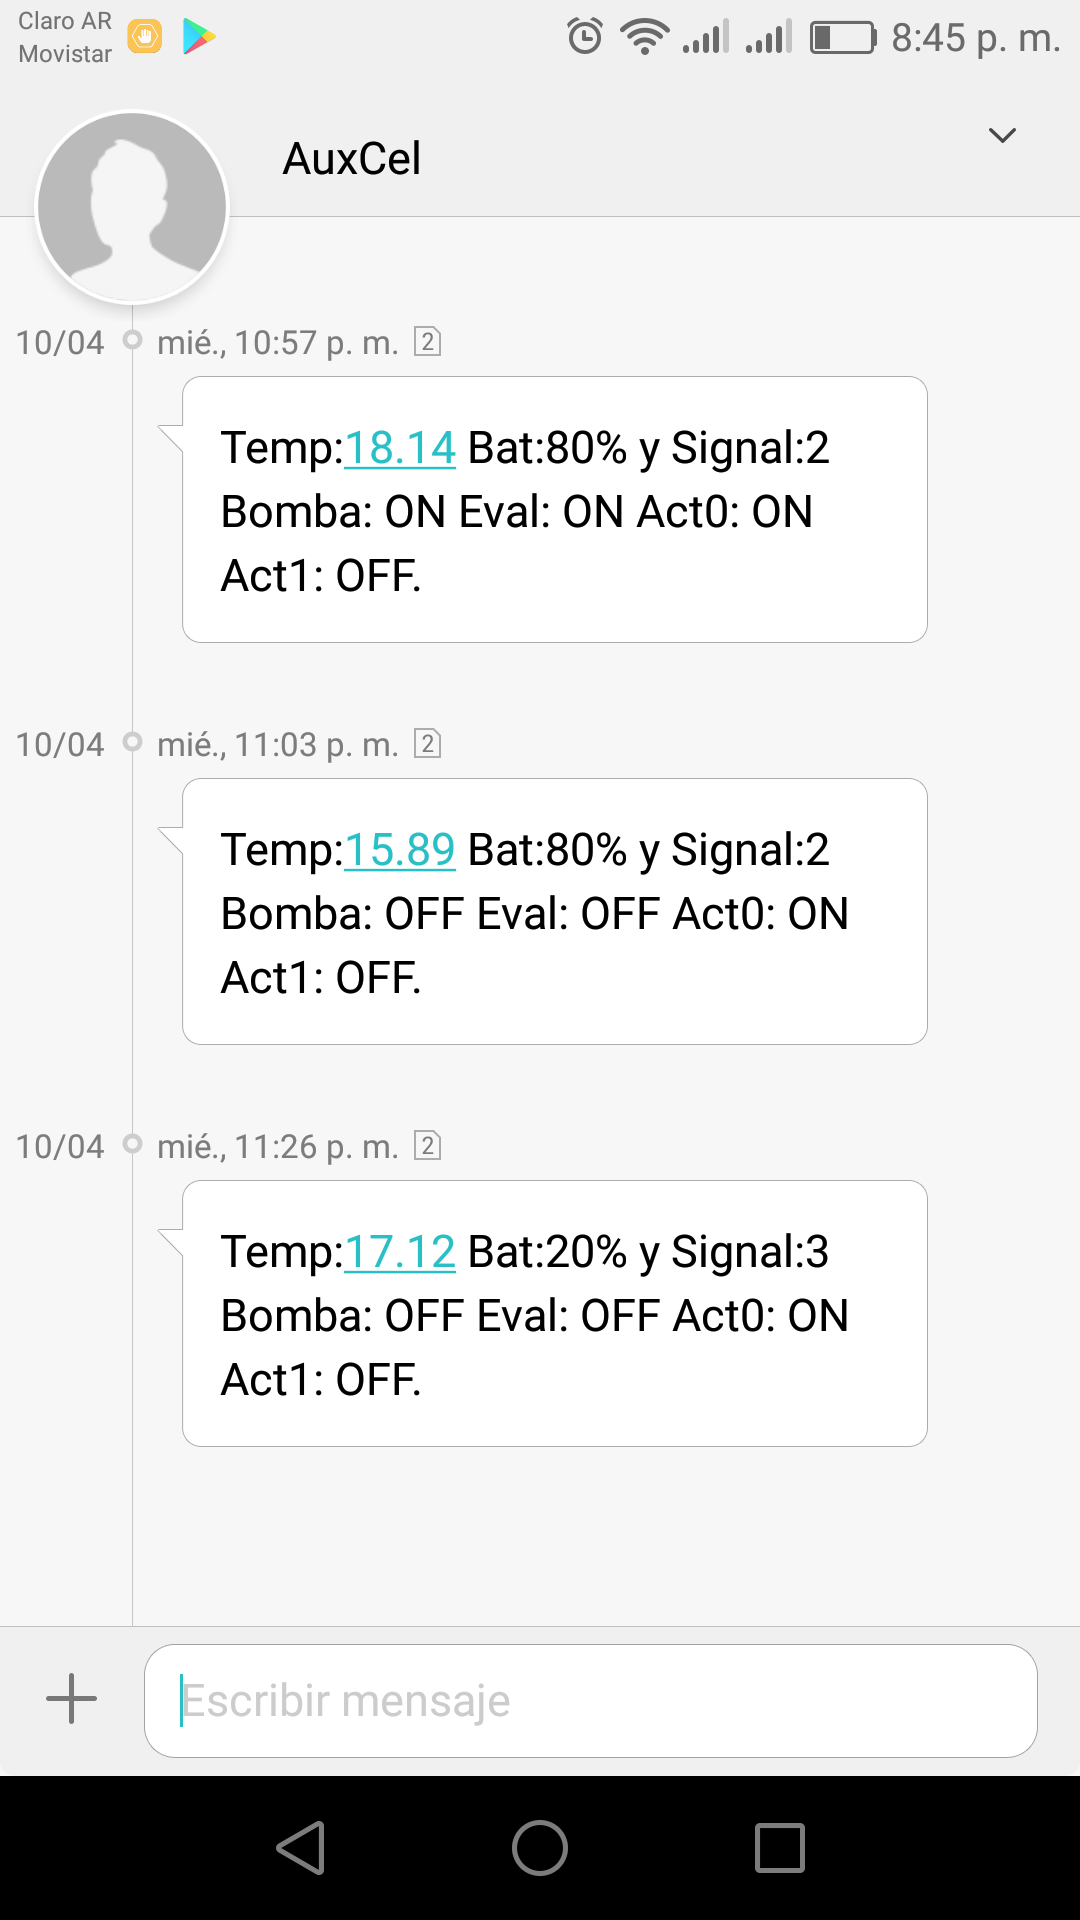
\includegraphics[scale=.15]{./Figures/sms_min_max_bat.png}
  \caption{SMS recibidos debido a temperatura máxima. \\
   El segundo SMS recibido es por temperatura mínima. \\
   Y el último recibido debido a bateria baja.}
  \label{fig:sms_min_max_bat}
\end{figure}

Se verificó que éste se mantiene activado hasta llegar a la temperatura mínima, en este instante procede a desconectar la bomba y a cerrar la electroválvula. En la web se verá como en la figura \ref{fig:auto_control_inactive}. y dado su respectiva alerta mediante un SMS como vemos en la figura \ref{fig:sms_min_max_bat}

\begin{figure}[h]
  \centering
  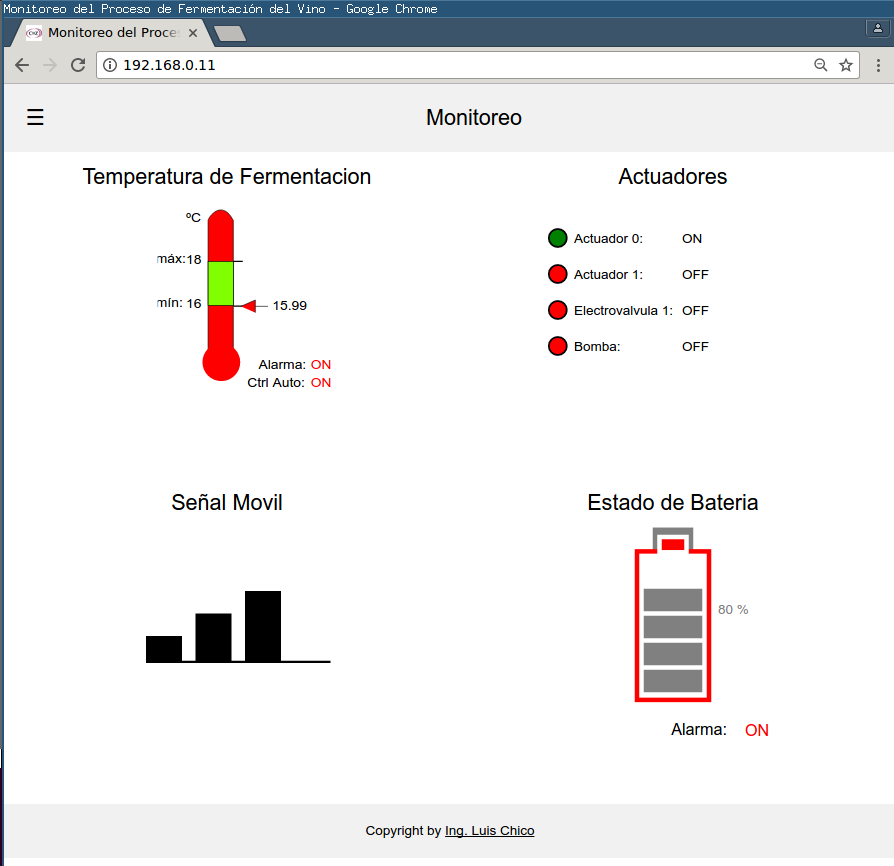
\includegraphics[scale=.25]{./Figures/auto_control_inactive.png}
  \caption{Temperatura en nivel mínimo, se desactiva la bomba y la electroválvula.}
  \label{fig:auto_control_inactive}
\end{figure}


En el caso de la batería se analíza las variaciones en la carga. Si esta disminuye más de un valor que es determinado, se enviará SMS como el que observamos en figura \ref{fig:sms_min_max_bat}. 

Para verificar los actuadores nos dirigimos a la web en la sección de configuración de actuadores y seteamos para cada uno de ellos los diferentes estados, encendiendo y apagando. Luego se probó en bloques de varios actuadores. En la siguiente figura \ref{fig:test_contact} se ve un ejemplo de los casos probados.

\begin{figure}[h]
  \centering
  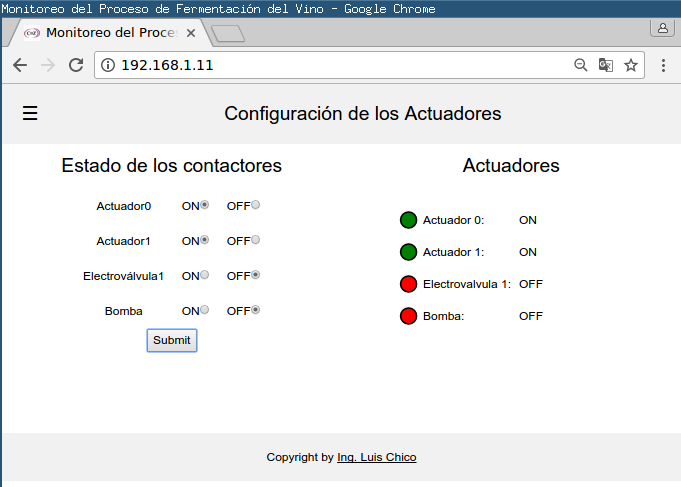
\includegraphics[scale=.25]{./Figures/test_contact.png}
  \caption{Activación manual de actuador 1 y 2, electroválvula y bomba inactivo.}
  \label{fig:test_contact}
\end{figure}


De esta forma podemos concluir que el funcionamiento del sistema es el correcto.





